\chapter{Job 38}

\begin{figure}
  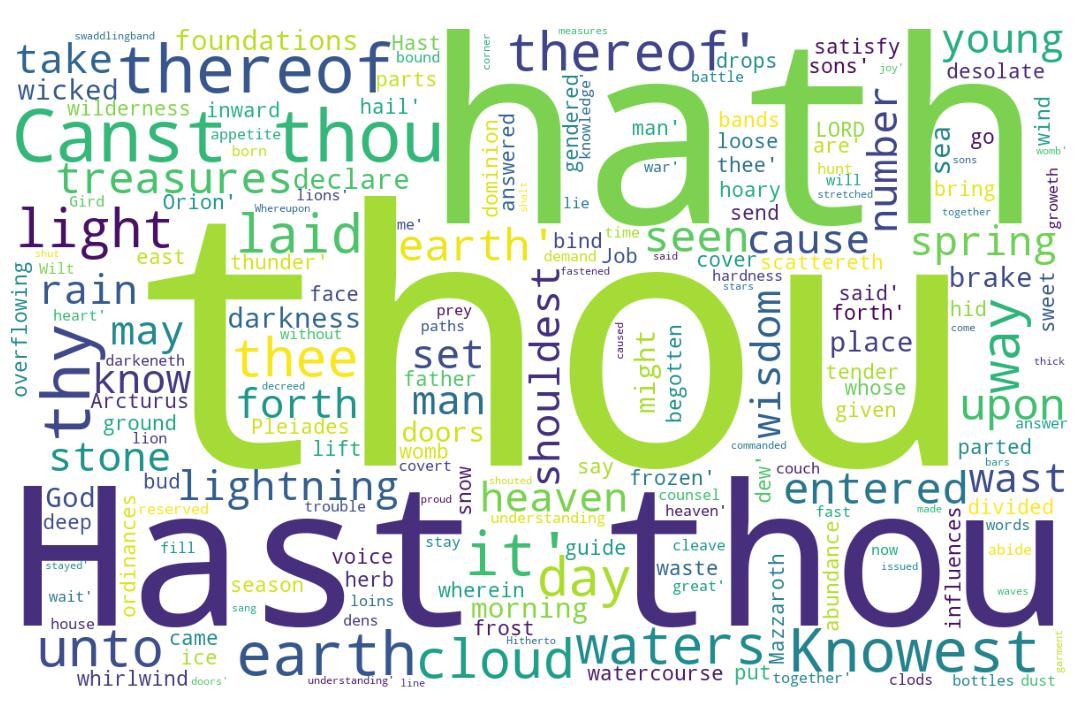
\includegraphics[width=\linewidth]{18OT-Job/Job38-WordCloud.jpg}
  \caption{Job 38 Word Cloud}
  \label{fig:Job 38 word Cloud}
\end{figure}

\marginpar{\scriptsize \centering \fcolorbox{bone}{lime}{\textbf{GOD IN CHARGE}}\\ (Job 38:1-41) \begin{compactenum}[I.][8]
    \item An \textbf{Appointment} %\index[scripture]{Job!Job 19:02}(Job 19:2)
    \item An \textbf{Accounting} \index[scripture]{Job!Job 38:02}(Job 38:2)
    \item \textbf{Answers} \index[scripture]{Job!Job 38:01} \index[scripture]{Job!Job 38:03}  (Job 38:1, 3)
    \item The \textbf{Authorship} \index[scripture]{Job!Job 38:05}(Job 38:5)
    \item The \textbf{Arrangement} \index[scripture]{Job!Job 38:06}(Job 38:6)
    \item The \textbf{Administration} %\index[scripture]{Job!Job 38:02}(Job 38:2)
    \item The \textbf{Attention} \index[scripture]{Job!Job 38:41}(Job 38:41)
\end{compactenum}}

\footnote{\textcolor[cmyk]{0.99998,1,0,0}{\hyperlink{TOC}{Return to end of Table of Contents.}}}\footnote{\href{https://www.audioverse.org/english/audiobibles/books/ENGKJV/O/Job/1}{\textcolor[cmyk]{0.99998,1,0,0}{Job  Audio}}}\textcolor[cmyk]{0.99998,1,0,0}{Then the LORD answered Job out of the whirlwind, and said,}
[2] \textcolor[cmyk]{0.99998,1,0,0}{Who \emph{is} this that darkeneth counsel by \fcolorbox{bone}{lime}{words} without knowledge?}
[3] \textcolor[cmyk]{0.99998,1,0,0}{Gird up now thy loins like a man; for I will demand of thee, and \fcolorbox{bone}{lime}{answer} thou me.}
[4] \textcolor[cmyk]{0.99998,1,0,0}{Where wast thou when I laid the foundations of the earth? declare, if thou hast \fcolorbox{bone}{MYGOLD}{understanding}.}\footnote{\textbf{Psalm 11:3} - If the foundations be destroyed, what can the righteous do?}\footnote{\textbf{Psalm 18:7} - Then the earth shook and trembled; the foundations also of the hills moved and were shaken, because he was wroth}\footnote{\textbf{Psalm 18:15} - Then the channels of waters were seen, and the foundations of the world were discovered at thy rebuke, O LORD, at the blast of the breath of thy nostrils.}\footnote{\textbf{Psalm 82:5} - They know not, neither will they understand; they walk on in darkness: all the foundations of the earth are out of course.}\footnote{\textbf{Psalm 104:5} - Who laid the foundations of the earth, that it should not be removed for ever.}\footnote{\textbf{Isaiah 24:18} - And it shall come to pass, that he who fleeth from the noise of the fear shall fall into the pit; and he that cometh up out of the midst of the pit shall be taken in the snare: for the windows from on high are open, and the foundations of the earth do shake.}
[5] \textcolor[cmyk]{0.99998,1,0,0}{\fcolorbox{bone}{lime}{Who} hath laid the measures thereof, if thou knowest? \fcolorbox{bone}{bone}{or} who hath stretched the line upon it?}
[6] \textcolor[cmyk]{0.99998,1,0,0}{Whereupon are the foundations thereof fastened? \fcolorbox{bone}{bone}{or} who laid the \fcolorbox{bone}{lime}{corner stone} thereof;}
[7] \textcolor[cmyk]{0.99998,1,0,0}{When the morning stars sang together, and all the sons of God shouted for joy?}
[8] \textcolor[cmyk]{0.99998,1,0,0}{Or \emph{who} shut up the sea with doors, when it brake forth, \emph{as} \emph{if} it had issued out of the womb?}
[9] \textcolor[cmyk]{0.99998,1,0,0}{When I made the cloud the garment thereof, and thick darkness a \fcolorbox{bone}{MYGOLD}{swaddlingband} for it,}
[10] \textcolor[cmyk]{0.99998,1,0,0}{And brake up for it my decreed \emph{place}, and set bars and doors,}
[11] \textcolor[cmyk]{0.99998,1,0,0}{And said, Hitherto shalt thou come, but no further: and here shall thy proud waves be stayed?}
[12] \textcolor[cmyk]{0.99998,1,0,0}{Hast thou commanded the morning since thy days; \emph{and} caused the dayspring to know his place;}
[13] \textcolor[cmyk]{0.99998,1,0,0}{That it might take hold of the ends of the earth, that the wicked might be shaken out of it?}
[14] \textcolor[cmyk]{0.99998,1,0,0}{It is turned as clay \emph{to} the seal; and they stand as a garment.}
[15] \textcolor[cmyk]{0.99998,1,0,0}{And from the wicked their light is withholden, and the high arm shall be broken.}
[16] \textcolor[cmyk]{0.99998,1,0,0}{Hast thou entered into the springs of the sea? \fcolorbox{bone}{bone}{or} hast thou walked in the search of the depth?}
[17] \textcolor[cmyk]{0.99998,1,0,0}{Have the gates of death been opened unto thee? \fcolorbox{bone}{bone}{or} hast thou seen the doors of the shadow of death?}
[18] \textcolor[cmyk]{0.99998,1,0,0}{Hast thou perceived the breadth of the earth? declare if thou knowest it all.}
[19] \textcolor[cmyk]{0.99998,1,0,0}{Where \emph{is} the way \emph{where} light dwelleth? and \emph{as} \emph{for} darkness, where \emph{is} the place thereof,}
[20] \textcolor[cmyk]{0.99998,1,0,0}{That thou shouldest take it to the bound thereof, and that thou shouldest know the paths \emph{to} the house thereof?}
[21] \textcolor[cmyk]{0.99998,1,0,0}{Knowest thou \emph{it}, because thou wast then born? \fcolorbox{bone}{bone}{or} \emph{because} the number of thy days \emph{is} great?}
[22] \textcolor[cmyk]{0.99998,1,0,0}{Hast thou entered into the treasures of the snow? \fcolorbox{bone}{bone}{or} hast thou seen the treasures of the hail,}
[23] \textcolor[cmyk]{0.99998,1,0,0}{Which I have reserved against the time of trouble, against the day of battle and war?}
[24] \textcolor[cmyk]{0.99998,1,0,0}{By what way is the light parted, \emph{which} scattereth the east wind upon the earth?}
[25] \textcolor[cmyk]{0.99998,1,0,0}{Who hath divided a watercourse for the overflowing of waters, \fcolorbox{bone}{bone}{or} a way for the lightning of thunder;}
[26] \textcolor[cmyk]{0.99998,1,0,0}{To cause it to rain on the earth, \emph{where} no man \emph{is;} \emph{on} the wilderness, wherein \emph{there} \emph{is} no man;}
[27] \textcolor[cmyk]{0.99998,1,0,0}{To satisfy the desolate and waste \emph{ground}; and to cause the bud of the tender herb to spring forth?}
[28] \textcolor[cmyk]{0.99998,1,0,0}{Hath the rain a father? \fcolorbox{bone}{bone}{or} who hath begotten the drops of dew?}
[29] \textcolor[cmyk]{0.99998,1,0,0}{Out of whose womb came the ice? and the hoary frost of heaven, who hath gendered it?}
[30] \textcolor[cmyk]{0.99998,1,0,0}{The waters are hid as \emph{with} a stone, and the face of the deep is frozen.}\footnote{\textbf{Genesis 1:2} - And the earth was without form, and void; and darkness was upon the face of the deep. And the Spirit of God moved upon the face of the waters.}
[31] \textcolor[cmyk]{0.99998,1,0,0}{Canst thou bind the sweet influences of Pleiades, \fcolorbox{bone}{bone}{or} loose the bands of Orion?}
[32] \textcolor[cmyk]{0.99998,1,0,0}{Canst thou bring forth Mazzaroth in his season? \fcolorbox{bone}{bone}{or} canst thou guide Arcturus with his sons?}
[33] \textcolor[cmyk]{0.99998,1,0,0}{Knowest thou the ordinances of heaven? canst thou set the dominion thereof in the earth?}
[34] \textcolor[cmyk]{0.99998,1,0,0}{Canst thou lift up thy voice to the clouds, that abundance of waters may cover thee?}
[35] \textcolor[cmyk]{0.99998,1,0,0}{Canst thou send lightnings, that they may go, and say unto thee, Here we \emph{are}?}
[36] \textcolor[cmyk]{0.99998,1,0,0}{Who hath put wisdom in the inward parts? \fcolorbox{bone}{bone}{or} who hath given \fcolorbox{bone}{MYGOLD}{understanding} to the heart?}
[37] \textcolor[cmyk]{0.99998,1,0,0}{Who can number the clouds in wisdom? \fcolorbox{bone}{bone}{or} who can stay the bottles of heaven,}
[38] \textcolor[cmyk]{0.99998,1,0,0}{When the dust groweth into hardness, and the clods cleave fast together?}
[39] \textcolor[cmyk]{0.99998,1,0,0}{Wilt thou hunt the prey for the lion? \fcolorbox{bone}{bone}{or} fill the appetite of the young lions,}
[40] \textcolor[cmyk]{0.99998,1,0,0}{When they couch in \emph{their} dens, \emph{and} abide in the covert to lie in wait?}
[41] \textcolor[cmyk]{0.99998,1,0,0}{Who \fcolorbox{bone}{lime}{provideth} for the raven his food? when his young ones cry unto God, they wander for lack of meat.}